\documentclass[border=3pt]{standalone}
% Preâmbulo compartilhado pelos diagramas TikZ da aula 5 de IHC (Processos de Design)
\usepackage[T1]{fontenc}
\usepackage[utf8]{inputenc}
\usepackage{lmodern}
\usepackage{amsmath}
\usepackage{xcolor}
\usepackage{tikz}
\usetikzlibrary{arrows.meta,angles,quotes,decorations.pathmorphing,calc,
                positioning,shapes.geometric,shapes.misc,backgrounds,fit,
                math}

% Paleta (mesma dos SVGs originais)
% Paleta da disciplina de IHC: acento roxo (#755099), da capa do livro.
% (o nome "dblue" é mantido para não alterar todos os diagramas)
\definecolor{dblue}{HTML}{755099}
\definecolor{dorange}{HTML}{B3541E}
\definecolor{dgreen}{HTML}{4A7C59}
\definecolor{dred}{HTML}{9C4B4B}
\definecolor{dcream}{HTML}{F4F1EA}
\definecolor{dshade}{HTML}{DDD7C9}

% Função gaussiana (não normalizada por padrão de escala visual)
\pgfmathdeclarefunction{gauss}{3}{%
  \pgfmathparse{1/(#3*sqrt(2*pi))*exp(-((#1-#2)^2)/(2*#3^2))}%
}

% Estilos comuns (prefixo d... para não colidir com chaves internas do pgf)
\tikzset{
  >={Stealth[length=2mm]},
  dguide/.style={gray!55, dashed, line width=0.4pt},
  daxis/.style={gray!60, line width=0.7pt, ->},
  dbody/.style={fill=black!3, draw=black!80, line width=1pt},
  dacc/.style={draw=dblue, line width=1pt},
  dlbl/.style={black!55, font=\small},
  dsub/.style={black!45, font=\footnotesize},
  dstate/.style={circle, draw=black!80, fill=dcream, line width=1pt,
                 minimum size=17mm, font=\large, inner sep=1pt},
  dobs/.style={circle, draw=black!80, fill=dshade, line width=1pt,
               minimum size=14mm, font=\large, inner sep=1pt},
  dbox/.style={rounded corners=2pt, draw=black!80, fill=dcream, line width=1pt,
               align=center, inner sep=6pt},
  dop/.style={circle, draw=black!80, fill=white, line width=1pt,
              minimum size=6mm, inner sep=0pt, font=\small},
  dtrans/.style={->, dblue, line width=1pt},
  dmeas/.style={->, dorange, line width=1pt},
  dcurve/.style={line width=1pt, dblue},
  dcurveb/.style={line width=1.4pt, dorange},
}

\begin{document}
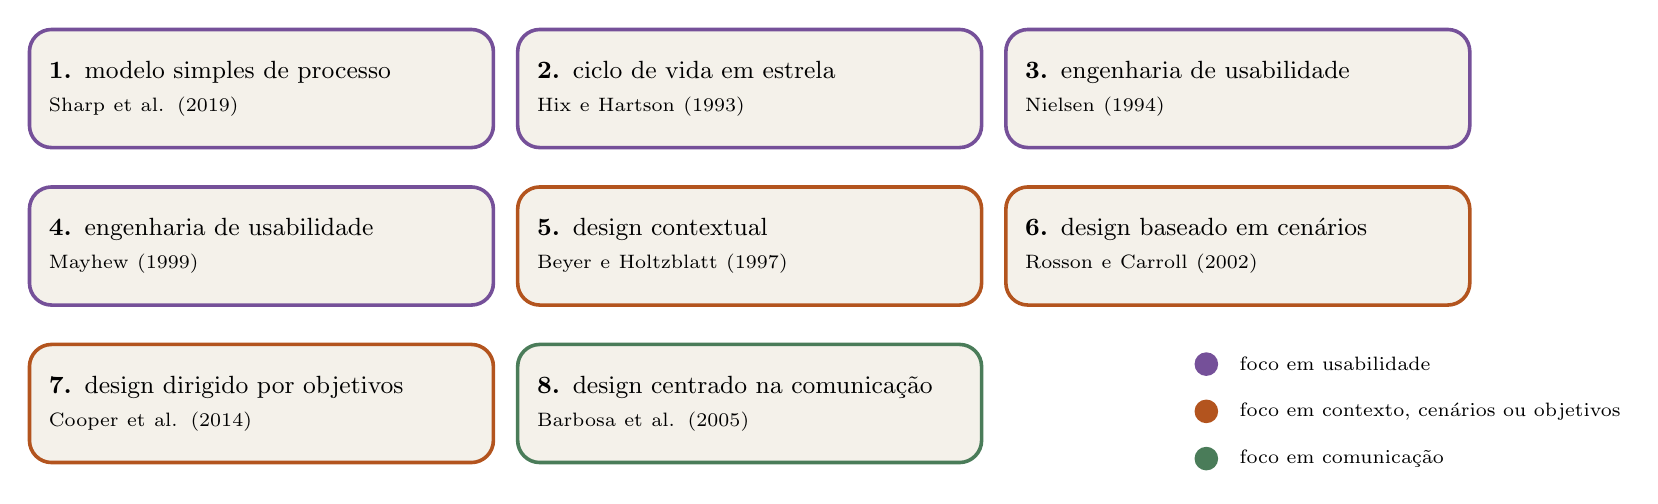
\begin{tikzpicture}[x=1cm,y=1cm,
   pr/.style={dbox, rounded corners=8pt, text width=5.4cm, minimum height=1.5cm, font=\small, align=left, inner sep=7pt}]

  \node[pr, draw=dblue, line width=1.3pt] at (0,0) {\textbf{1.} modelo simples de processo\\[1pt] {\scriptsize Sharp et al. (2019)}};
  \node[pr, draw=dblue, line width=1.3pt] at (6.2,0) {\textbf{2.} ciclo de vida em estrela\\[1pt] {\scriptsize Hix e Hartson (1993)}};
  \node[pr, draw=dblue, line width=1.3pt] at (12.4,0) {\textbf{3.} engenharia de usabilidade\\[1pt] {\scriptsize Nielsen (1994)}};
  \node[pr, draw=dblue, line width=1.3pt] at (0,-2.0) {\textbf{4.} engenharia de usabilidade\\[1pt] {\scriptsize Mayhew (1999)}};
  \node[pr, draw=dorange, line width=1.3pt] at (6.2,-2.0) {\textbf{5.} design contextual\\[1pt] {\scriptsize Beyer e Holtzblatt (1997)}};
  \node[pr, draw=dorange, line width=1.3pt] at (12.4,-2.0) {\textbf{6.} design baseado em cenários\\[1pt] {\scriptsize Rosson e Carroll (2002)}};
  \node[pr, draw=dorange, line width=1.3pt] at (0,-4.0) {\textbf{7.} design dirigido por objetivos\\[1pt] {\scriptsize Cooper et al. (2014)}};
  \node[pr, draw=dgreen, line width=1.3pt] at (6.2,-4.0) {\textbf{8.} design centrado na comunicação\\[1pt] {\scriptsize Barbosa et al. (2005)}};

  \fill[dblue] (12.0,-3.5) circle (0.15); \node[anchor=west, font=\scriptsize] at (12.3,-3.5) {foco em usabilidade};
  \fill[dorange] (12.0,-4.1) circle (0.15); \node[anchor=west, font=\scriptsize] at (12.3,-4.1) {foco em contexto, cenários ou objetivos};
  \fill[dgreen] (12.0,-4.7) circle (0.15); \node[anchor=west, font=\scriptsize] at (12.3,-4.7) {foco em comunicação};

\end{tikzpicture}
\end{document}
